In this chapter we show the algorithms and definitions that compose our
abstraction model for the verification of neural networks by means of
reachability analysis and robustness certification. We give the general 
definitions for abstracting domains, and afterwards we focus on how to 
propagate this abstraction throughout the activation layers.

\section{Basic abstraction definitions}
\label{sec:abstr}

To enable algorithmic verification of neural networks, we consider the
abstract domain $\langle \mathbb{R}^n \rangle \subset 2^{\mathbb{R}^n}$ 
of polytopes defined in $\mathbb{R}^n$ to abstract (families of) bounded
sets into (families of) polytopes. We provide corresponding
abstractions for affine and functional layers to perform abstract
computations and we prove that their composition provides a consistent
overapproximation of concrete networks.

\begin{definition}{(Abstraction)}
\label{def:abs}
\normalfont Given a bounded set $X \subset \mathbb{R}^n$,
an abstraction is defined as a function $\alpha : 2^{\mathbb{R}^n} \to
\langle \mathbb{R}^n \rangle$
that maps $X$ to a polytope $P$ such
that $\mathcal{C}(X) \subseteq P$.
\end{definition}

Intutively, the function $\alpha$ maps a bounded set $X$ to a
corresponding polytope in the abstract space such that the polytope
always contains the convex hull of $X$. Depending on $X$, the
enclosing polytope may not be unique --- see Figure~\ref{fig:exabs}
for different examples. However, given the convex hull of any bounded
set, it is always possible to find an enclosing polytope. As shown
in~\cite{zheng2019computing}, one could always start with 
an axis-aligned regular $n$ simplex consisting of $n+1$ facets ---
e.g., the
triangle in $\mathbb{R}^2$ and the tethraedron in $\mathbb{R}^3$ ---
and then refine the abstraction as needed by adding facets, i.e.,
adding half-spaces to make the abstraction more precise. 

\begin{definition}{(Concretization)}
\label{def:concr}
\normalfont Given a polytope $P \in \langle \mathbb{R}^n \rangle$
a concretization is a function $\gamma : \langle \mathbb{R}^n \rangle
\to 2^{\mathbb{R}^n}$ that maps $P$ to the set of points cointained in
it, i.e., $\gamma(P) = \{ x \in \mathbb{R}^n \mid x \in P \}$.
\end{definition}

Intutively, the function $\gamma$ simply maps a polytope $P$ to the
corresponding (convex and compact) set in $\mathbb{R}^n$ 
comprising all the points contained in the polytope. As opposed to
abstraction, the result of concretization is uniquely determined.
We extend abstraction and concretization to finite families of
sets and polytopes, respectively, as follows. Given a family of $p$
bounded sets $\Pi = \{X_1, \ldots, X_p \}$, the abstraction of $\Pi$
is a set of polytopes $\Sigma = \{P_1, \ldots, P_s\}$ such that
$\alpha(X_i) \subseteq \bigcup_{i=1}^s P_i$ for all $i \in [1,p]$;
when no ambiguity arises, we abuse notation and write $\alpha(\Pi)$ to
denote the abstraction corresponding  to the family $\Pi$. Given a
family of $s$ polytopes $\Sigma = \{P_1, \ldots, P_s\}$, the
concretization of $\Sigma$ is the union of the concretizations of its
elements, i.e., $\bigcup_{i=1}^s \gamma(P_i)$; also in this case, we
abuse notation and write $\gamma(\Sigma)$ to denote the concretization
of a family of polytopes $\Sigma$.

\begin{figure}[t]
	\centering
	\caption{\label{fig:exabs} Three possible abstractions of a
		set: the first row depicts the bounded set $X$, and the second
		the enclosing polytope $P$. Starting from the left, the first
		set is a convex set whose polytope matches perfectly. The second
		is not linear, and it is approximated with an octagon. The third
		is linear but non convex, therefore is split into two convex
		polytopes.}
	\begin{tabular}{ccc}
		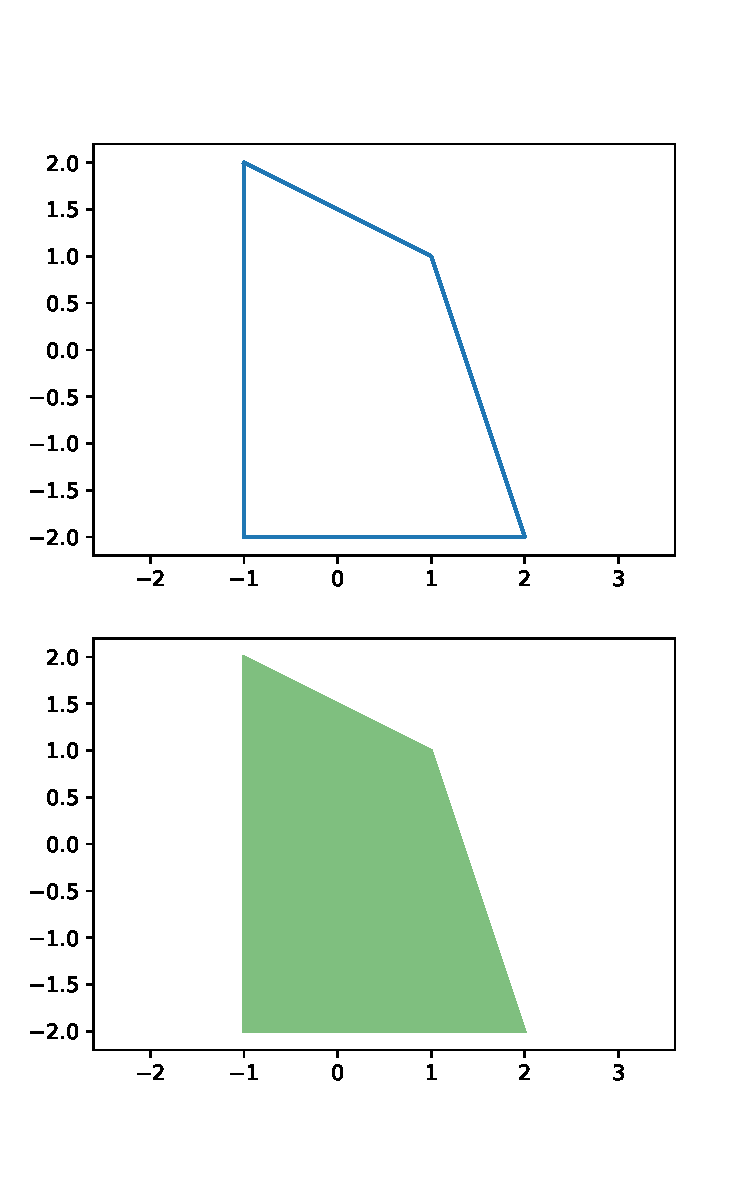
\includegraphics[width=.3\linewidth]{NN/input1_convex.pdf} &
		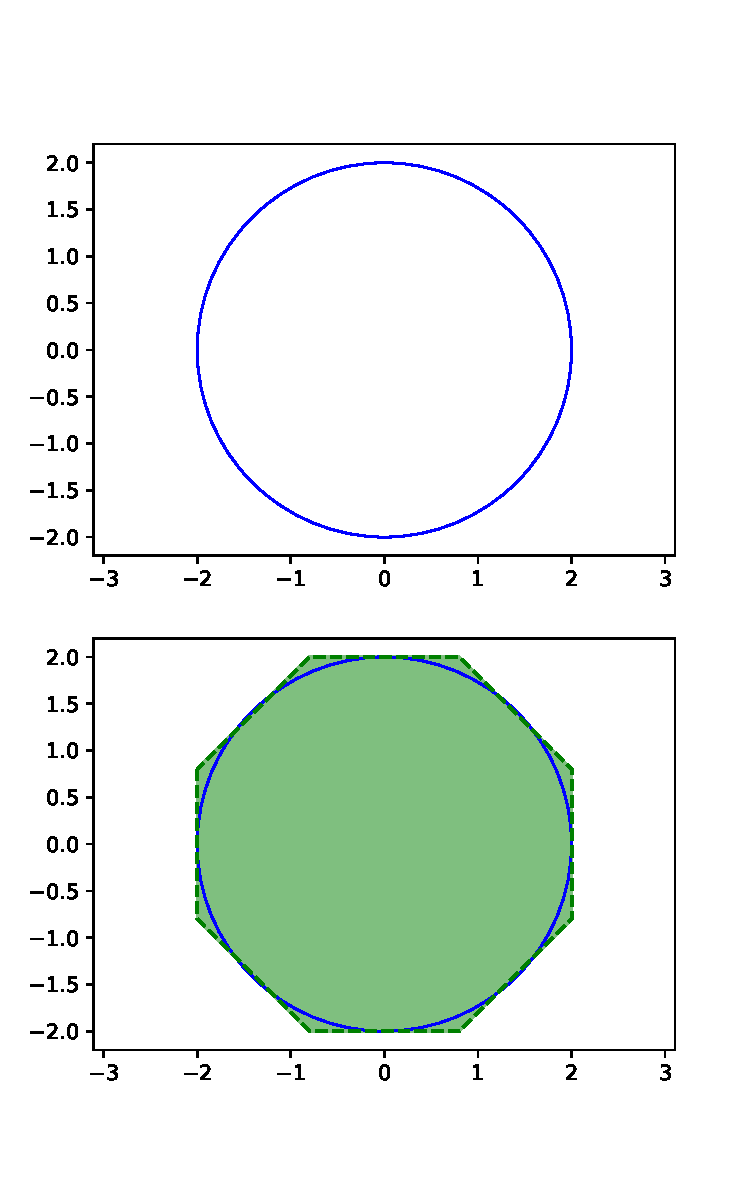
\includegraphics[width=.3\linewidth]{NN/input2_approx.pdf} &
		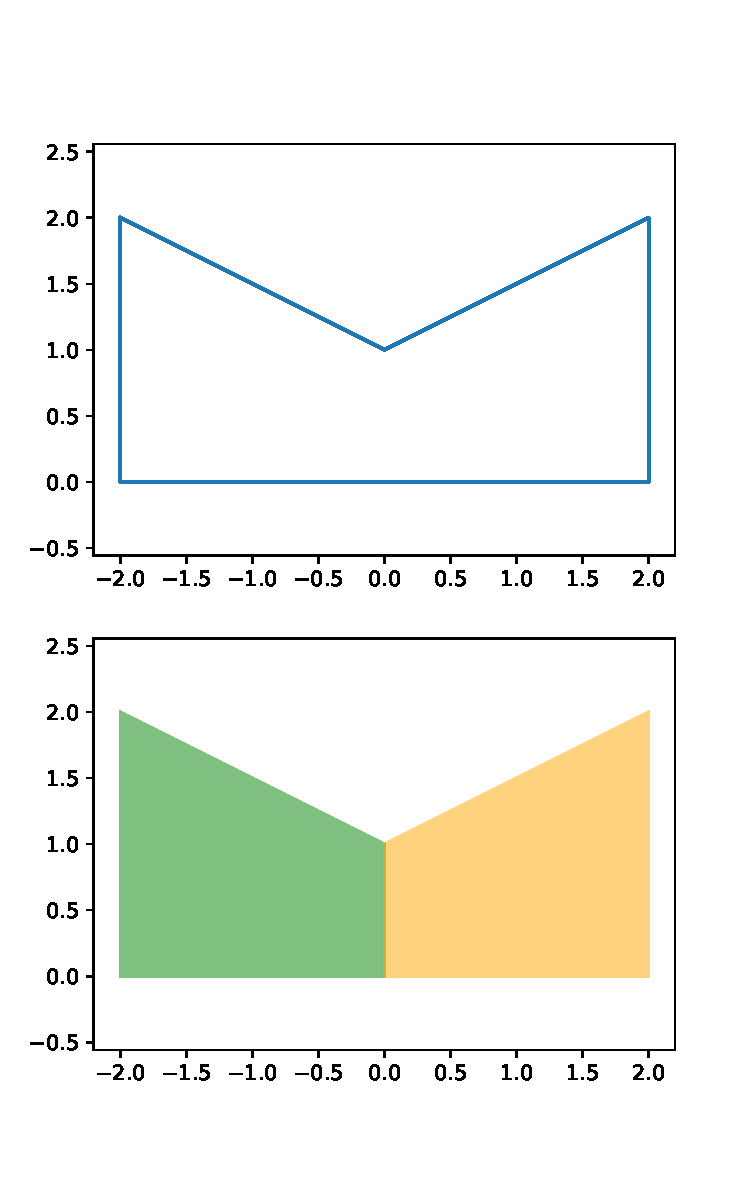
\includegraphics[width=.3\linewidth]{NN/input3_split.pdf}
	\end{tabular}
\end{figure}

Given our choice of abstract domain and a concrete network $\nu :
I \to O$ with $I \subset \mathbb{R}^n$ and $O \subset \mathbb{R}^m$,
we need to show how to obtain an \emph{abstract neural network}
$\tilde{\nu} : \langle I \rangle \to \langle O \rangle$ that provides
a sound overapproximation of $\nu$. To frame this concept, we
introduce the notion of consistent abstraction.

\begin{definition}{(Consistent abstraction)}
\normalfont Given a mapping $\nu : \mathbb{R}^n \to \mathbb{R}^m$, a 
mapping $\tilde{\nu} : \langle \mathbb{R}^n \rangle \to \langle 
\mathbb{R}^m \rangle$, abstraction function $\alpha : 2^{\mathbb{R}^n} 
\to \langle \mathbb{R}^m \rangle$ and concretization function 
$\gamma : \langle \mathbb{R}^m \rangle \to 2^{\mathbb{R}^m}$,
the mapping $\tilde{\nu}$ is a consistent abstraction of $\nu$ over a 
set of inputs $X \subseteq I$ exactly when 
\begin{equation}
\label{eq:cons}
\{ \nu(x) \mid x \in X \} \subseteq \gamma(\tilde{\nu}(\alpha(X)))
\end{equation}
\end{definition}

The notion of consistent abstraction can be readily extended to
families of sets as follows. The mapping $\tilde{\nu}$ is a consistent
abstraction of $\nu$ over a family of sets of inputs $X_1 \ldots X_p$
exactly when 
\begin{equation}
\label{eq:consset}
\{ \nu(x) \mid x \in \cup_{i=1}^p X_i \} \subseteq
\gamma(\tilde{\nu}(\alpha(X_1, \ldots, X_p)))
\end{equation}
where we abuse notation and denote with $\tilde{\nu}(\cdot)$
the family 
$\{ \tilde{\nu}(P_1), \ldots, \tilde{\nu}(P_s) \}$ with
$\{P_1, \ldots, P_s\} = \alpha(X_1, \ldots X_p)$

To represent polytopes and define the computations performed by
abstract layers we resort to a specific subclass of \emph{generalized star
sets}, introduced in~\cite{bak2017simulation} and defined as
follows --- the notation is adapted from~\cite{tran2019star}.

\begin{definition}{(Generalized star set)}
  \normalfont Given a \emph{basis matrix}
  $V \in \mathbb{R}^{n \times m}$ obtained arranging a set of
  $m$ \emph{basis vectors} $\{v_1, \ldots v_m\}$ in columns , a point
  $c \in \mathbb{R}^n$ called \emph{center} and a \emph{predicate} $R 
  : \mathbb{R}^m \to \{\top, \bot\}$, a generalized star set is a
  tuple $\Theta = (c,V,R)$.
  The set of points represented by the generalized star set is given by 
  \begin{equation}
    [ \! [ \Theta  ] \! ]  \equiv \{z \in \mathbb{R}^n \mid z = Vx + c
    \mbox{ such that } R(x_1, \ldots, x_m) = \top\}
  \end{equation}
\end{definition}

In the following we denote $[\![ \Theta ]\!]$ also as
$\Theta$. Depending on the choice of $R$, generalized star sets can
represent different kinds of sets, but 
we consider only those such that $R(x) := Cx \leq d$, where $C \in
\mathbb{R}^{p \times m}$ and $d \in \mathbb{R}^p$ for $p \geq 1$,
i.e., $R$ is a conjunction of $p$ linear constraints
as in~\cite{tran2019star}; we further require that the set $Y = \{y \in
\mathbb{R}^m \mid C y \leq  d\}$ is bounded. 

\begin{proposition}
\label{prop:polistar}
Given a generalized star set $\Theta = (c,V,R)$ such that
$R(x) := Cx \leq d$ with $C \in \mathbb{R}^{p \times m}$ and
$d \in \mathbb{R}^p$, if the set $Y
= \{y \in \mathbb{R}^m \mid C y \leq d\}$ is bounded, then the set of
points represented by  $\Theta$ is a polytope in $\mathbb{R}^n$, i.e.,
$\Theta \in \langle \mathbb{R}^n \rangle$. 
\end{proposition}

The proof of proposition (\ref{prop:polistar}) is
straightforward, since the set $Y$ is a polytope in $\mathbb{R}^m$, 
the mapping  $Vx + c$ is an affine mapping from  $\mathbb{R}^m$ to
$\mathbb{R}^n$ and affine mappings of polytopes are still
polytopes. From~\cite{tran2019star} we know that polytopes can be
represented as generalized star sets, and thus our 
restricted form of star sets provides an equivalent representation  
of polytopes in $\mathbb{R}^n$; in the following, we refer
to generalized star sets obeying our restrictions simply as \emph{stars}.

The simplest abstract layer to obtain is the one abstracting affine
transformations. As we have already mentioned, affine transformations
of polytopes are still polytopes, so we just need to define how to
apply an affine transformation to a star --- the definition is
adapted from~\cite{tran2019star}.  

\begin{definition}
  \label{def:absaffine} (Abstract affine mapping)
  \normalfont Given a star set $\Theta = (c,V,R)$ and an affine
  mapping $f : R^n \to R^m$ with $f = Ax + b$, the abstract affine
  mapping $\tilde{f} : \langle R^n \rangle \to \langle R^m \rangle$
  of $f$ is defined as $\tilde{f}(\Theta) = (\hat{c},\hat{V},R)$ where 
  \begin{equation*}
    \hat{c} = Ac + b \qquad \hat{V} = AV 
  \end{equation*}
\end{definition}

Intuitively, the center and the basis vectors of the input star
$\Theta$ are affected by the transformation of $f$, while the
predicates remain the same.

\begin{proposition}
\label{prop:affinecons}
Given an affine mapping $f : \mathbb{R}^n \to \mathbb{R}^m$, the
corresponding abstract mapping $\tilde{f} : \langle
\mathbb{R}^n \rangle \to \langle \mathbb{R}^m \rangle$ provides a consistent
abstraction over any bounded set $X \subset \mathbb{R}^n$, i.e.,
$\{ f(x) \mid x \in X \} \subseteq \gamma(\tilde{f}(\alpha(X)))$ for
all $X \subset \mathbb{R}^n$. 
\end{proposition}

To prove proposition (\ref{prop:affinecons}), we observe that
the set $\alpha(X)$ is any polytope $P$ such that $P \supseteq \mathcal{C}(X)$
--- equality holds only when $X$ is already a polytope, and thus $X
\equiv \mathcal{C}(X) \equiv P$. Let $\Theta_P = (c_P,V_P,R_P)$ be the
star corresponding to $P$ defined as
\begin{equation*}
c_P = 0^n \qquad V_P = I^n \qquad R_P = C_Px + d_P \leq 0
\end{equation*}
where $0^n$ is the $n$-dimensional zero vector, and $I^n$ is the $n
\times n$ identity matrix --- the columns of $I^n$ correspond
to the standard orthonormal basis $e_1, \ldots, e_n$ of
$\mathbb{R}^n$, i.e., $\lVert e_i \rVert = 1$ and $e_i \cdot e_j = 0$
for all $i \neq j$ with $i,j \in [1,n]$; the matrix $C_P \in
\mathbb{R}^{q \times n}$ and the vector $d_P \in 
\mathbb{R}^q$ collect the parameters defining $q$ half-spaces
whose intersection corresponds to $P$. Given our choice of $c$ and
$V$, it is thus obvious that $\Theta_P \equiv P$. Recall that $f = Ax + b$
with $A \in \mathbb{R}^{m \times n}$ and $b \in \mathbb{R}^m$; from  
definition (\ref{def:absaffine}) we have that
$\tilde{f}(\Theta_P) = \hat{\Theta}_P$ with $\hat{\Theta}_P = (\hat{c}_P, \hat{V}_P, R_P)$ and
\begin{equation*}
\hat{c}_P = A 0^n + b = b \qquad \hat{V}_P = AI^n = A
\end{equation*}
The concretization of $\hat{\Theta}_P$ is just the set of
points contained in $\hat{\Theta}_P$ defined as
\begin{equation}
  \label{eq:affineconc}
\gamma(\hat{\Theta}_P) = \{ z \in \mathbb{R}^m \mid z = Ax  + b
\mbox{ such that } C_px \leq d_P \}
\end{equation}
Now it remains to show that $\{ f(x) \mid x \in X \} \subseteq
\gamma(\hat{\Theta}_P)$. This follows from the fact that, for a generic $y
\in \{ f(x) \mid x \in X \}$ there must exists $x \in X$ such that $y
= Ax + b$; since $x$ satisfies $C_p x \leq d_P$ by construction of
$P$, it is also the case that $y \in \gamma(\hat{\Theta}_P)$ by definition
(\ref{eq:affineconc}).

\section{ReLU abstraction algorithms}
\label{sec:relu_abst}

\begin{algorithm}[t!]
  \caption{Abstraction of the ReLU activation function.}
  \label{alg:relu-abst}
  \small
  \begin{algorithmic}[1]
    \Function{compute\_layer}{\emph{input} = $[\Theta_1, \ldots, \Theta_N]$, \emph{refine} = $[r_1, \ldots, r_n]$}
    \State \emph{output} = $[\:]$
    \For{$i = 1:N$} 
      \State \emph{stars} = $[\Theta_i]$
      \For{$j$ = $1:n$}
        \emph{stars} = \textsc{compute\_relu}(\emph{stars}, $j$,
        \emph{refine}$[j]$, $n$)
      \EndFor
      \State \textsc{append}(\emph{output}, \emph{stars})
    \EndFor
    \State \Return \emph{output}
    \EndFunction
  \item[]
    \Function{compute\_relu}{\emph{input} = $[\Gamma_1, \ldots,
        \Gamma_M]$, $j$, \emph{level}, $n$}
    \State $output$ = $[\: ]$
    \For{$k = 1:M$}
      \State $(lb_j, ub_j)$ = \textsc{get\_bounds}(\emph{input}$[k]$, $j$)
      \State $M = [e_1\ ...\ e_{j-1}\ 0\ e_{j+1}\ ...\ e_n]$
      \If {$lb_j \geq 0$} $S$ = \emph{input}$[k]$
      \ElsIf {$ub_j \leq 0$} $S$ = $M$ * \emph{input}$[k]$
      \Else
        \If{\emph{level} $>$ $0$}
          \State $\Theta_{low}$ = \emph{input}$[k] \wedge z[j] < 0$;
          \hspace{1ex}$\Theta_{upp}$ = \emph{input}$[k] \wedge z[j] \geq 0$
          \State $S$ = $[M \mbox{ * } \Theta_{low}, \Theta_{upp}]$
        \Else
          \State $(c,V,Cx \leq d)$ = \emph{input}$[j]$
          \State $C_1$ = $[0\ 0\ ...\ -1] \in \mathbb{R}^{1 \times m+1}$, $d_1 = 0$
          \State $C_2$ = $[V[j,:]\ -1] \in \mathbb{R}^{1 \times m+1}$, $d_2 = -c_k[j]$
          \State $C_3$ = $[\frac{-ub_j}{ub_j - lb_j} \cdot V[j,:]\ -1] \in \mathbb{R}^{1 \times m+1}$, $d_3 = \frac{ub_j}{ub_j - lb_j} (c[j] - lb_j)$
          \State $C_0$ = $[C\ 0^{m \times 1}]$, $d_0 = d$
          \State $\hat{C}$ = $[C_0;\ C_1;\ C_2;\ C_3]$, $\hat{d} = [d_0;\ d_1;\ d_2;\ d_3]$
          \State $\hat{V} = MV$, $\hat{V} = [\hat{V}\ e_j]$
          \State $S$ = $(Mc, \hat{V}, \hat{C} \hat{x} \leq \hat{d})$
        \EndIf
      \EndIf
      \State \textsc{append}($output$, S)
    \EndFor
    \State \Return $output$
    \EndFunction
  \end{algorithmic}
\end{algorithm}

Algorithm~\ref{alg:relu-abst}~\cite{guidotti2021pynever} defines 
the abstract mapping of a functional layer with $n$ ReLU activation 
functions and adapts the methodology proposed in~\cite{tran2019star}. 
The function \textsc{compute\_layer} takes as input an indexed list 
of $N$ stars $\Theta_1, \ldots, \Theta_N$ and an indexed list of $n$ 
positive integers called \emph{refinement levels}. For each neuron, 
the refinement level tunes the grain of the abstraction: level $0$
corresponds to the coarsest abstraction that we consider --- the
greater the level, the finer the abstraction grain. In the case of
ReLUs, all non-zero levels map to the same (precise) refinement, i.e.,
a piecewise affine mapping. The output of function
\textsc{compute\_layer} is still an indexed list of stars, that can be
obtained by independently processing the stars in the input list.
For this reason, the \textbf{for} loop starting at line 3
can be  parallelized to speed up actual implementations. 

Given a single input star $\Theta_i \in \langle R^n \rangle$, each 
of the $n$ dimensions is processed in turn by the \textbf{for} loop 
starting at line 5 and involing the function \textsc{compute\_relu}. 
Notice that the stars obtained processing the $j$-th dimension are 
feeded again to \textsc{compute\_relu} in order to process the 
$j+1$-th dimension. For each star given as input, the
function \textsc{compute\_relu} first computes the lower and upper
bounds of the star along the $j$-th dimension by solving two
linear-programming problems --- function \textsc{get\_bounds} at line
11. Independently from the abstraction level, if $lb_j \geq 0$ then
the ReLU acts as an identity function (line 13), whereas if $ub_j \leq
0$ then the $j$-th dimension is zeroed (line 14). The $\ast$ operator
takes a matrix $M$, a star $\Gamma = (c, V, R)$ and returns the star
$(Mc, MV, R)$. In this case, $M$ is composed of the standard orthonormal
basis in $\mathbb{R}^n$ arranged in columns, with the exception of 
the $j$-th dimension which is zeroed. 

\subsection{Exact abstract propagation}

When $lb_j < 0$ and $ub_j > 0$ we consider the refinement level. 
For any non-zero level, the input star is ``split” into two new stars, 
one considering all the points $z < 0$ ($\Theta_{low}$) and the other 
considering points $z \geq 0$ ($\Theta_{upp}$) along dimension $j$. 
Both $\Theta_{low}$ and $\Theta_{upp}$ are obtained by adding to the 
input star \textit{input[k]} the appropriate constraints. 
If the analysis at lines 17–18 is applied throughout the network, 
and the input abstraction is precise, then the abstract output 
range will also be precise, i.e., it will coincide with the concrete one: 
we call complete the analysis of \nevertwo{} in this case. The number
of resulting stars is worst-case exponential, therefore the complete
analysis may result computationally infeasible.

\begin{proposition}
\label{prop:relucons}
Given a ReLU mapping $f : \mathbb{R}^n \to \mathbb{R}^n$, the
corresponding abstract mapping $\tilde{f} : \langle
\mathbb{R}^n \rangle \to \langle \mathbb{R}^n \rangle$ defined in 
Algorithm~\ref{alg:relu-abst} provides a consistent 
abstraction over any bounded set $X \subset \mathbb{R}^n$, i.e.,
$\{ f(x) \mid x \in X \} \subseteq \gamma(\tilde{f}(\alpha(X)))$ for
all $X \subset \mathbb{R}^n$. 
\end{proposition}

%\textbf{TODO: proof of the above}

\begin{proposition}
\label{prop:allcons}
Given a concrete network $\nu : \mathbb{R}^n \to \mathbb{R}^m$ comprised 
of a finite number $p$ of layers 
$f_1: \mathbb{R}^n  \to \mathbb{R}^{n_1}, \ldots, f_p: \mathbb{R}^{n_{p-1}} \to \mathbb{R}^{m}$ 
such that each $f_i$ is either an affine or functional layer implementing 
ReLUs, the corresponding abstract network
$\tilde{\nu} : \langle \mathbb{R}^n \rangle \to \langle \mathbb{R}^m \rangle$ 
comprised of the corresponding abstract layers 
$\tilde{f}_1: \langle \mathbb{R}^n \rangle  \to \langle \mathbb{R}^{n_1} \rangle, \ldots, 
\tilde{f}_p: \langle \mathbb{R}^{n_{p-1}} \rangle \to \langle \mathbb{R}^{m} \rangle$ 
provides a consistent abstraction over any bounded set $X \subset \mathbb{R}^n$, i.e.,
$\{ \nu(x) \mid x \in X \} \subseteq \gamma(\tilde{\nu}(\alpha(X)))$ for
all $X \subset \mathbb{R}^n$. 
\end{proposition}

Proposition~\ref{prop:allcons} enforces that we can prove the (local) robustness of
a neural network by propagating the abstraction of an input set representing the
$l_{\infty}$ ball around a given input with a small perturbation $\epsilon$ and check
whether the output set is large enough to cause a misclassification.

\begin{proposition}
\label{prop:halfspace-intersect}
The intersection of a star $\Theta = (c,V,R)$ and a half-space 
$\mathcal{H} = \{z | Hz \leq g\}$ is another star with the following characteristics:
$\overline{\Theta} = \Theta \cap \mathcal{H} = (\overline{c},\overline{V},
\overline{R})$ with $\overline{c} = c$, $\overline{V} = V$,
$\overline{R} = R \wedge R'$ and $R'(x) = (H V)x \leq g - H c$
\end{proposition}
The proof of the proposition is straightforward since it is analogous to 
adding new constraints to the predicate of the star, as done for the ReLU 
abstract transformer.

\begin{proposition}
\label{prop:safety}
Let $[\Theta_1, ..., \Theta_n]$ be a star set obtained by applying 
Algorithm~\ref{alg:relu-abst} to a network of interest $\nu$ and an input star set 
corresponding to the input component of the property of interest $P$. Moreover let 
$\mathcal{\hat{H}}$ be an half-space corresponding to the unsafe zone as defined 
by the property of interest. 
If $\overline{\Theta}_i = \Theta_i \wedge \mathcal{\hat{H}} = \emptyset$ for $i = 1, ..., n$ 
then the neural network $\nu$ satisfy the property $P$.
\end{proposition}

\begin{proposition}
\label{prop:counter-input-set}
If in Algorithm~\ref{alg:relu-abst} the stars were always refined for all 
neurons it is possible to compute the complete counter input set 
(\textit{i.e.}, the set containing all possible inputs that make the neural 
network unsafe) as $\mathcal{C}_{\Theta} = \bigcup_i (c, V, \overline{R}_i)$ 
where $\overline{R}_i$ are the predicates of the stars obtained by the 
intersection between the unsafe zone and the output star set, whereas $c$ 
and $V$ are the center and basis matrix of the input star. 
\end{proposition}

\begin{proof}
\label{proof:counter-input-set}
If the complete version of Algorithm~\ref{alg:relu-abst} is used then all 
the stars in the computation process are defined on the same predicate variables
$\textbf{x} = [x_1, ..., x_m]$ which do not change during the computations since 
only the number of constraints on $\textbf{x}$ is changed by the abstract
transformers. As consequence the $\overline{R}_i$ contain values of $\textbf{x}$ 
that make the network unsafe, moreover it also contains all the constraints of
the base predicate $R$ of the input star. Therefore the complete counter input 
set containing all possible inputs that make the neural network unsafe is
$\mathcal{C}_{\Theta} = \bigcup_i (c, V, \overline{R}_i)$, $\overline{R}_i \neq \emptyset$.
\end{proof}

\subsection{Over-approximate abstract propagation}
\label{subsec:relu-overapprox}

If the refinement level is $0$, then the ReLU is abstracted using 
the over-approximation proposed in~\cite{tran2019star} and 
depicted in Figure~\ref{fig:relu-overapprox}. This approach is 
much less conservative than others, i.e., based on zonotopes or 
abstract domains, and provides a tighter abstraction.

\begin{figure}
	\centering
	\caption{\label{fig:relu-overapprox} Graphical representation
		of the ReLU function (left) and the over-approximation 
		considering a single variable (right) with $lb_{j} = -2$ 
		and $ub_{j} = 2$.}
	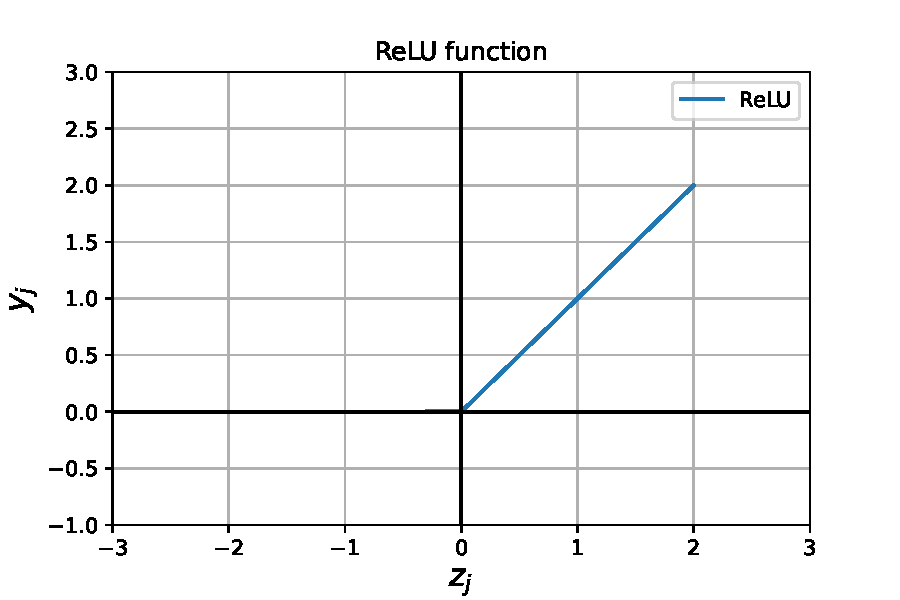
\includegraphics[width=.48\textwidth]{NN/ReLU_figure.pdf}
	\hspace*{\fill}
	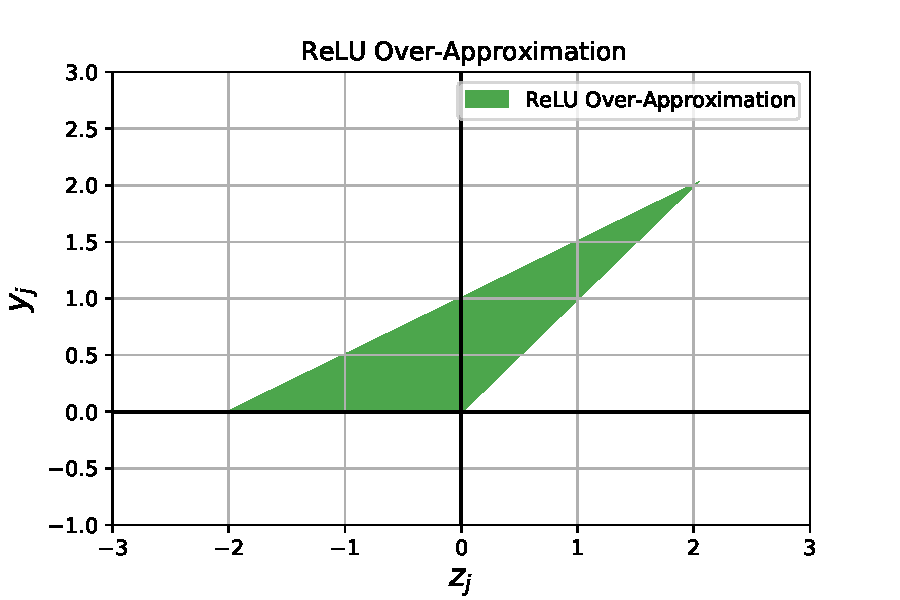
\includegraphics[width=.48\textwidth]{NN/relu_overapprox.pdf}
\end{figure}

As can be seen in Figure~\ref{fig:relu-overapprox}, three constraints
are needed to construct the over-approximation:
\begin{align*}
y_j &\geq 0\\
y_j &\geq z_j\\
y_j &\leq ub_j \frac{z_j - lb_j}{ub_j - lb_j}
\end{align*}
Such constraints must be added to the predicate matrix of the star, 
therefore we define an auxiliarly variable $x_{m+1}$ and we modify 
the basis matrix so that $y_j = x_{m+1}$ (line 26 in 
Algorithm~\ref{alg:relu-abst}). By doing so we make it possible to 
express our constraints only in terms of the predicate variables.
We remember that $z_j = V_j \mathbf{x} + c_j$, substituting it in 
the constraints we obtain:
\begin{align*}
x_{m+1} &\geq 0\\
x_{m+1} &\geq V_j \mathbf{x} + c_j\\
x_{m+1} &\leq ub_j \cdot \frac{V_j \mathbf{x} + c_j - lb_j}{ub_j - lb_j}
\end{align*}
If we reorder these constraints we can bring them in the format
$C\mathbf{x} \leq \mathbf{d}$:
\begin{align*}
- x_{m+1} &\leq 0\\
V_j \mathbf{x} - x_{m+1} &\leq -c_j\\
- \frac{ub_j}{ub_j-lb_j} V_j \mathbf{x} + x_{m+1} &\leq \frac{ub_j}{ub_j-lb_j}(c_j - lb_j)\\
\end{align*}
From these constraints it is straightforward to identify the 
corresponding matrices in lines 21 to 23 of the algorithm.

If this analysis is carried out throughout the network, then the 
output star will be a (sound) over-approximation of the concrete output 
range: we call \textit{over-approximate} the analysis of \nevertwo{} 
in this case. The number of star remains the same throughout
the analysis, but at the cost of a new predicate variable for each neuron
which, in turn, increases the complexity of the linear program required
by \textsc{get\_bounds}.

\subsection{Mixed abstract propagation}

In~\cite{guidotti2021pynever} it is proposed a new approach that adopts 
different levels of abstraction during the analysis: since each neuron
features its own refinement level, algorithm~\ref{alg:relu-abst}
controls the abstraction down to the single neuron. This setting strikes
a trade-off between complete and over-approximate settings. In order to
reduce as much as possible the approximation error, we rank the
neurons in each layer based on the area of the over-approximation
triangle depicted in Figure~\ref{fig:relu-overapprox}: intuitively,
the neuron with the widest bounds introduces a broader triangle and,
by design, a bigger approximation. 

We concretize the star along that neuron and propagate the approximate 
method along the others, such that each layer results in at most a single 
split. This reduces the computational cost significantly, as the growth 
becomes quadratic in the number of layers and the complexity increase by 
the approximation is contained. We call \textit{mixed} the analysis of 
\nevertwo{} in this case.